\documentclass[UTF8,fontset=fandol,11pt,a4paper]{ctexart}

\usepackage{fontspec}
\usepackage{amsmath,amssymb}
\usepackage{booktabs}
\usepackage{array}
\usepackage{enumitem}
\usepackage{float}
\usepackage{graphicx}
\usepackage{microtype}
\usepackage[numbers,sort&compress]{natbib}
\usepackage{xcolor}
\usepackage{xurl}
\usepackage{hyperref}

\hypersetup{
  colorlinks=true,
  linkcolor=blue!55!black,
  citecolor=blue!55!black,
  urlcolor=blue!55!black,
  pdftitle={多轮 RAG 何时停止？Search-R1 中的结构化停止判断与检索节省}
}

\setlength{\emergencystretch}{3em}
\newcommand{\model}[1]{\texttt{#1}}

\title{多轮 RAG 何时停止？\\Search-R1 中的结构化停止判断与检索节省}
\author{Weimeng Luo\\
\small Independent Researcher\\
\small \href{mailto:weimengluo@gmail.com}{weimengluo@gmail.com}}
\date{}

\begin{document}
\maketitle

\begin{abstract}
多轮检索增强生成（RAG）的停止决策不是独立状态上的二分类，而是序列选择问题。本文将 S2G-RAG 中“同时判断证据是否充分以及还缺什么”的结构化 Judge 机制适配到冻结的 Search-R1 流程，并使用 900 个互斥 HotpotQA 训练问题、3,009 个状态，专门训练一个 Qwen3.5-2B S2G 式 Judge；Search-R1 的 Reasoner、Retriever、语料、prompt 与搜索预算均保持不变。200 题探索性可达性审计显示，523 次原生搜索动作中有 143 次发生在冻结 answer-only probe 已可正确作答之后；质量 Oracle 将 EM 提高 5.0 个百分点，保持 Native EM 的成本 Oracle 可删除 25.05\% 的搜索。checkpoint 与阈值只在 grouped validation 上选择并冻结，最终在确认性测试集上评测。实验开始前规定，新策略相对 Native Search-R1 的 Official EM 下降最多允许 2 个百分点。实际 EM 仅下降 0.625 个百分点（差值 $-0.00625$；95\% CI $[-0.01250,0]$），未超过这一可接受范围；与此同时，检索减少 77 次，平均搜索下降 0.09625（3.70\%；95\% CI $[-0.12000,-0.07375]$）。因此，实验支持的主要结论是：为 Search-R1 训练的 S2G 式结构化 Judge 能在答案准确率下降不超过预设可接受范围的前提下减少检索调用。该结论不表示答案准确率完全不变或有所提高；69 次提前停止中仍有 27 次不安全，也不能据此声称停止安全或总体推理成本更低。
\end{abstract}

\noindent\textbf{关键词：}多轮检索增强生成；自适应检索；停止策略；风险—覆盖率；结构化 Judge；Search-R1

\section{引言}

迭代检索允许语言模型在推理过程中决定还需要什么证据。IRCoT 交替执行检索与链式推理 \citep{trivedi2023ircot}；Self-RAG 学习检索与反思控制 \citep{asai2023selfrag}；Adaptive-RAG 按问题复杂度选择不同检索策略 \citep{jeong2024adaptiverag}；Search-R1 则通过强化学习训练语言模型进行推理和搜索调用 \citep{jin2025searchr1}。灵活的检索轨迹同时引入停止难题：停止过早会留下证据或推理缺口，停止过晚会增加延迟与调用成本，新增上下文还可能把原本正确的候选答案改错。

SIM-RAG 将是否继续搜索建模为显式决策 \citep{yang2025simrag}；S2G-RAG 同时判断证据充分性与缺失信息 \citep{li2026s2grag}；TASR 研究无需训练的迭代检索停止 \citep{kieback2026tasr}；RAG-Critic 用 Critic 反馈引导 agentic workflow \citep{dong2025ragcritic}。这些工作证明停止器值得研究，但状态级分类指标或最终平均准确率并不能单独解释在线策略。

原因在于首次越界。分类器在大量中间状态上评估，而在线系统只执行每条轨迹中第一个越过阈值的 STOP。一个早期假阳性会截断全部后续状态；一个过度保守的高 AP 模型则可能完全不改变系统。此外，如果冻结轨迹中没有任何状态能够生成正确答案，调整停止时间也无法挽救该题。

本文回答四个问题：强搜索策略有多少搜索发生在答案已可恢复之后；冻结接口上的质量与成本上界有多大；结构化缺口监督能否改善状态排序和 earliest-stop 策略；确认性搜索节省伴随何种答案风险。论文贡献包括：将 S2G 式结构化 Judge 机制适配到 Search-R1，并基于 Search-R1 状态专门训练 Qwen3.5-2B Judge；提出候选可达性、状态排序、首次越界、端到端质量和成本的联合审计框架；展示“AP 改善但系统退化”的排序—策略失配；以及在确认性测试集上显示该完整策略能在答案准确率下降不超过预设可接受范围的前提下减少搜索。安全停止仍未得到证明。

\section{相关工作与论文定位}

\subsection{自适应检索接口}

自适应检索至少包含四种不同接口。问题级 router 在轨迹开始前选择不检索、单次检索或多步检索 \citep{jeong2024adaptiverag}；交替式系统在推理中决定下一条查询 \citep{trivedi2023ircot,jin2025searchr1}；生成式控制在生成过程中触发检索或反思 \citep{asai2023selfrag}；答案级控制器则接受已有候选或继续搜索 \citep{yang2025simrag}。不同接口的 Oracle、标签和错误语义不能直接互换。

本文冻结 Search-R1 的 Qwen2.5-7B PPO v0.2 Reasoner、E5 top-3 Retriever、Wiki-2018 语料、prompt 和四次搜索预算。唯一干预是是否提前接受冻结可达状态。因此，本文的 Oracle 是条件经验上界，不是所有可能查询、文档和模型上的理论上界。

\subsection{结构化 Judge 与风险—覆盖率}

本文采用 S2G-RAG 的核心机制假设：二元充分/不充分标签丢失了“还缺什么”的训练信号 \citep{li2026s2grag}。我们把这一结构化判断机制移植到 Search-R1 的状态接口，并在 Search-R1 状态上专门训练 Judge。Judge 输出固定 JSON schema，包含 \model{sufficient} 与 \model{gap\_items}；在线分数来自固定前缀处 true/false 的 log-prob margin。本文不声称复现完整 S2G-RAG 系统，也没有训练或修改 Search-R1 本身；研究对象是“冻结 Search-R1 + 训练后的 S2G 式 Judge”这一完整停止策略。

选择性分类把主动接受子集的条件错误率与 coverage 分开 \citep{geifman2017selective}，RAG 风险控制进一步强调生成风险的校准 \citep{kang2024crag}。本文沿用这种区分，但不提供风险认证。主要科学门只控制 EM 非劣与配对搜索减少；STOP precision、recall、AP、校准和端到端 EM 仍是不同结果。

\section{问题定义}

图~\ref{fig:stopping-framework-zh} 概括本文的论证链。可达候选决定停止器
可能达到的上界，状态分数只诊断排序能力，首次越界决定实际执行的停止，
最终还必须分别检验答案质量、所选 STOP 风险和检索成本。

\begin{figure}[t]
\centering
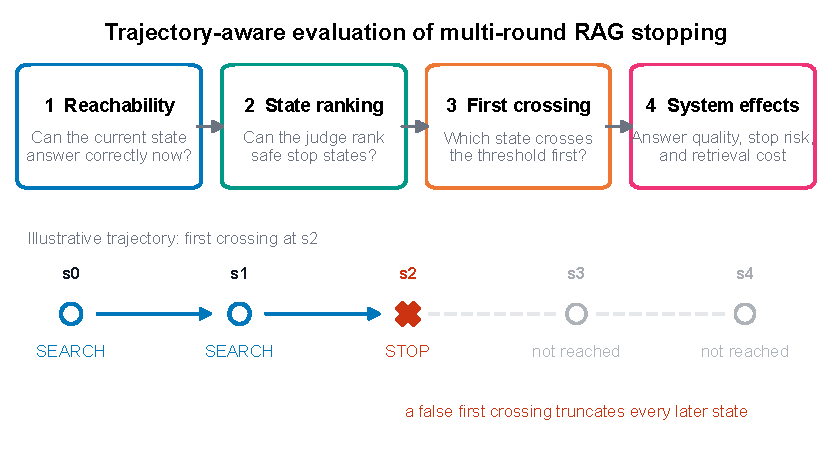
\includegraphics[width=\linewidth]{figures/stopping-evaluation-framework.pdf}
\caption{多轮 RAG 停止的轨迹级评测框架。正确候选可达只是必要条件；
Judge 还需正确排序，earliest crossing 必须先选中适当状态，且答案质量、
所选 STOP 风险与检索成本必须分别报告。}
\label{fig:stopping-framework-zh}
\end{figure}

对问题 $q_i$，Native Search-R1 产生冻结可达状态
\begin{equation}
z_{i,t}=(q_i,C_{i,t},h_{i,t},a^{\mathrm{native}}_{i,t}),
\end{equation}
其中 $C_{i,t}$ 是累积检索上下文，$h_{i,t}$ 是推理历史，$a^{\mathrm{native}}_{i,t}$ 是下一原生动作。本文在初始状态和每次成功检索后的状态运行冻结 answer-only probe $g$，得到候选 $\tilde a_{i,t}=g(q_i,C_{i,t})$。probe 输出不反馈给 Native 轨迹。

当候选按官方规范化规则与答案一致时，记 $y_{i,t}=1$。若 Native 下一动作仍为 SEARCH 且 $y_{i,t}=1$，则存在安全提前停止机会。该标签表示冻结 Answerer 已能恢复官方答案，不等价于 supporting-fact 意义上的证据完备。

质量 Oracle 后验选择每题最早的正确可达状态。Native-preserving 成本 Oracle 只对 Native 原本正确的问题提前停止，从而保持 Native EM 不变并估计最多可删除的检索。两者都使用 gold，因此只作诊断。

Judge 给出状态分数 $s_{i,t}$。阈值 $\theta$ 下的策略在
\begin{equation}
\tau_i(\theta)=\min\{t:s_{i,t}\geq\theta\}
\end{equation}
停止；若无越界状态，则执行冻结回退。状态级 AP 衡量排序，STOP precision/recall 衡量阈值判别，系统级 safe/unsafe early stop 衡量每题首个被选状态，Official EM 衡量全题质量，平均搜索次数衡量检索成本。配对区间使用 10,000 次问题级 bootstrap，seed 为 20260728。

\section{实验设计}

\subsection{上游系统与数据}

上游系统为官方 Search-R1 Qwen2.5-7B PPO v0.2 checkpoint、E5 top-3 和 Wiki-2018，最多搜索四次 \citep{jin2025searchr1}。独立的 1,200 题 NQ/HotpotQA 审计得到 45.67\%/46.00\% Official EM；论文参考值均落在来源级 Wilson 95\% 区间内且点差小于五个百分点。因此本文称其为“配置已核验且结果相容”，而非严格复现。

scale-up 使用 S2G-code-aligned HotpotQA distractor dev 前 1,000 题 \citep{yang2018hotpotqa}。训练、grouped validation、reserve 与 final 问题在 ID 和规范化题面上互斥。

\subsection{探索性可达性门禁}

Gate H0 复用 200 条冻结 Native 轨迹，包含 200 个初始状态和 523 个 Native SEARCH 前状态。另有 75 个 forced-continue 产生的反事实状态，只作补充，不归因为 Native。probe prompt、确定性解码、解析、去重与成本规则在 labels 不可见时冻结，798 个状态全部成功解析。由于这 200 题已用于早期 pilot，H0 只决定研究可行性，不支持最终系统结论。

\subsection{扩充版 S2G Judge}

HotpotQA train 按问题划分为 700 个 fresh train、100 个 grouped validation 和 200 个 reserve。依据预冻结的数据充分性门，最终训练使用 900 个问题、3,009 个 clean states。Teacher generation/schema 失败按冻结规则删除，不人工修复标签。Supporting-fact labels 仅在 Teacher 生成后用于单向强冲突过滤，不进入 Judge 输入。

Qwen3.5-2B 训练三轮、12,654 steps，所有 loss 有限且无训练 OOM。输出顶层键顺序冻结为 \model{sufficient} 后接 \model{gap\_items}。仅依据 grouped teacher-target token NLL 选择 epoch 1。扩充 adapter tree SHA-256 为 \nolinkurl{cfed584b95025cc4f1fd555cd2236b2773f1289c67dab03d26b2829659578767}。

对每个 Judge，grouped validation 在至少 10 个预测 STOP 且经验 precision 不低于 0.90 的前提下最大化 recall。无可行阈值时，冻结实现以“验证状态最大分数加一”的有限 sentinel 编码 \model{fallback=never\_stop}；该 sentinel 保证 grouped validation 上零 STOP，但不保证在新分布上严格永不停止。扩充版阈值约为 7.875，Structured Base 与旧 LoRA 均触发该保守回退，其 sentinel 分别为 2.5 和约 8.0。

indices 0--199 保持探索角色，200--999 构成确认性测试集。实验开始前规定，扩充版相对 Native 的 EM 最多允许下降 2 个百分点；统计判据是 EM 差的 95\% CI 下界高于 $-0.02$。同时，搜索差的 95\% CI 上界必须低于 0，才能判定检索确有减少。前一条件在统计上是非劣判据，通俗地说就是“答案准确率的下降不能超过预设可接受范围”；它不表示准确率完全不变。全 1,000 题只作描述性报告。

\section{结果}

\subsection{强搜索策略仍有可辨识的停止上界}

H0 中，523 次 Native SEARCH 有 143 次（27.3\%）发生在 probe 已正确作答之后，涉及 70/200 题。60 题为 cost-only over-search，10 题为早期正确但 Native 最终错误的 harmful over-search。Native EM 为 46.5\%，质量 Oracle 为 51.5\%，精确增量为 10/200=5.0 个百分点。保持 Native EM 的成本 Oracle 可删除 131/523（25.05\%）次搜索。

固定预算 $k=0,1,2,3,4$ 的 answer-only EM 分别为 18.5\%、34.0\%、43.0\%、46.0\% 和 47.0\%。统一预算不能实现问题级 Oracle，说明状态自适应控制具有研究空间。

\begin{figure}[t]
\centering
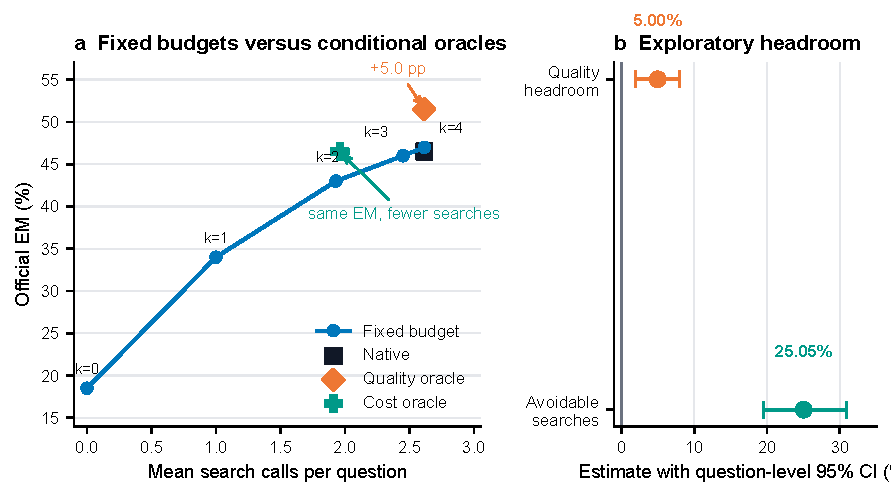
\includegraphics[width=\linewidth]{figures/h0-stopping-headroom.pdf}
\caption{200 题探索性 H0 停止余量。Panel (a) 比较统一搜索预算、Native
Search-R1 与两个依赖标签的条件 Oracle；Panel (b) 给出问题级 bootstrap
95\% 区间。质量 Oracle 为后验选择，成本 Oracle 保持 Native EM；二者均
不是可部署策略，也不是确认性结果。}
\label{fig:h0-headroom-zh}
\end{figure}

\subsection{排序改善不自动转化为策略改善}

Core200 机制诊断中，Binary LoRA 将 STOP AP 从 0.732 提高到 0.828，但零阈值策略把 Official EM 从 36.5\% 降到 31.5\%，平均搜索从 2.635 降到 1.430。更强的排序信号在激进阈值下导致过早停止。

最小 S2G 监督把 wrong STOP 从 99 降到 24、premature STOP 从 18 降到 4，EM 从 31.5\% 恢复到 35.5\%，平均搜索回升到 2.390。相对 Structured Base 的 EM 差仅为 $+0.015$，95\% CI $[-0.010,0.040]$。因此该阶段只支持“结构化缺口降低激进过停”的机制判断。

\subsection{Grouped validation 冻结策略}

100 个 grouped-validation 问题上，扩充 Judge 的 STOP precision/recall/AP 为 0.9091/0.1205/0.5285；Official EM 与 Native 均为 0.53，平均搜索从 2.45 降到 2.33。该结果只用于冻结 policy，不能与 final 后缀合并为确认性证据。

\subsection{确认性测试集：准确率降幅不超过预设范围，并减少搜索}

两个确认性判据均通过。在第 200--999 题组成的确认性测试集上，Native 的 EM 为 0.44875，平均搜索为 2.60125；扩充 S2G 的对应结果为 0.44250 和 2.50500。配对 EM 差为 $-0.00625$，95\% CI 为 $[-0.01250,0]$；也就是说，点估计下降 0.625 个百分点，统计区间仍未越过实验前规定的“最多下降 2 个百分点”界限。搜索差为 $-0.09625$，95\% CI 为 $[-0.12000,-0.07375]$；区间上界低于零。

按绝对计数，Native 在 800 题上执行 2,081 次检索，扩充策略执行 2,004 次，减少 77 次，即 3.70\%。答案结果有 6 题从 Native 正确变为扩充策略错误，1 题从 Native 错误变为扩充策略正确，净变化为 $-5/800=-0.625$ 个百分点。表~\ref{tab:suffix800-zh} 将效应量、区间和预冻结判据并列，避免把非劣解释成等价或优越。

\begin{table}[H]
\centering
\small
\caption{确认性测试集主要结果。差值定义为扩充 S2G 减 Native；两个预冻结判据均通过。}
\label{tab:suffix800-zh}
\resizebox{\linewidth}{!}{%
\begin{tabular}{lrrrll}
\toprule
指标 & Native & 扩充 S2G & 差值 [95\% CI] & 预冻结判据 & 结果 \\
\midrule
Official EM & 0.44875 & 0.44250 & $-0.00625\;[-0.01250,0]$ & CI 下界 $>-0.02$ & PASS \\
平均搜索 & 2.60125 & 2.50500 & $-0.09625\;[-0.12000,-0.07375]$ & CI 上界 $<0$ & PASS \\
\bottomrule
\end{tabular}
}
\end{table}

扩充版相对 Structured Base 的 STOP AP 差为 0.03983，95\% CI $[0.00571,0.07228]$，为结构化状态排序改善提供了确认性证据。但排序改善不等于提前停止安全。表~\ref{tab:suffix800-diagnostics-zh} 将状态级诊断与系统级首次停止分开报告。Structured Base 与旧 S2G 的有限 sentinel 在确认后缀上各被一个状态超过，故其实现是验证集相对的保守回退，而非数学意义上的无限阈值。

\begin{table}[H]
\centering
\small
\caption{确认性测试集 Judge 诊断。STOP P/R/AP 为全部 eligible states 的状态级指标；“提前停止（安全/不安全）”为每题首次越界的系统级计数。}
\label{tab:suffix800-diagnostics-zh}
\begin{tabular}{lrrrr}
\toprule
Judge & STOP P & STOP R & STOP AP & 提前停止（安全/不安全） \\
\midrule
Structured Base & 0.0000 & 0.0000 & 0.36375 & 1（0/1） \\
旧 S2G LoRA & 1.0000 & 0.0019 & 0.36596 & 1（1/0） \\
扩充 S2G LoRA & 0.6216 & 0.0880 & 0.40358 & 69（42/27） \\
\bottomrule
\end{tabular}
\end{table}

\subsection{搜索节省伴随实质风险}

扩充策略产生 69 次系统级提前停止，占 800 题的 8.63\%。其中 42 次安全、27 次不安全，所选提前停止的不安全比例为 39.13\%；42 次安全停止只覆盖 294 个存在安全机会问题中的 14.29\%。状态级 STOP precision 为 0.6216、recall 为 0.0880。42/69 是每题首次被选状态的系统口径，0.6216 是全部 eligible states 的阈值口径，二者不应混写。

grouped validation 的 STOP precision 为 0.9091，但只基于 11 个预测 STOP；冻结阈值在确认后缀上的状态级 precision 降至 0.6216。因此，验证阶段的 0.90 precision 没有迁移到最终分布。扩充版 Brier score 为 0.2952，十箱 ECE 为 0.2911；Structured Base 分别为 0.1992 和 0.1179。扩充版排序更好，但 raw score 校准更差。在状态级 precision 至少 0.90 的事后 operating point 上，recall 仅 0.0057。因此，本文不能把策略称为风险已认证或安全。

27 次不安全停止不与新增错误逐一对应。相对 Native，只有 6 题由正确变错，另有 1 题由错误变对；其余不安全停止发生在 Native 已错误的问题，或不满足冻结 safe-opportunity 定义但最终答案仍正确。EM 非劣门衡量全题平均质量，selected-stop risk 衡量策略主动接受的条件风险，二者回答不同问题，必须同时报告。

图~\ref{fig:confirmatory-tradeoff-zh} 将三个事实并置：EM 区间保持在冻结
非劣界之上，搜索差区间在有利方向排除零，但所选提前停止仍有实质不安全
比例。它同时表达本文的正面结果与最重要的主张边界。

\begin{figure}[t]
\centering
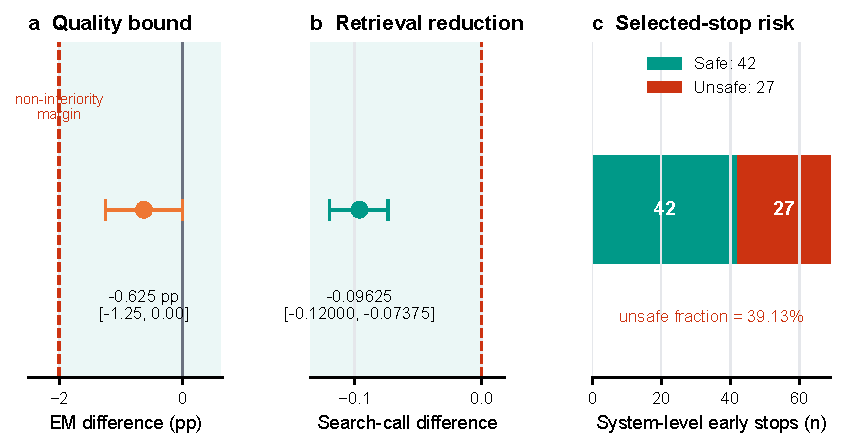
\includegraphics[width=\linewidth]{figures/confirmatory-quality-cost-risk.pdf}
\caption{扩充 S2G 相对 Native Search-R1 的确认性测试集质量—成本—
风险结果。Panels (a)(b) 为配对 bootstrap 95\% 区间，虚线分别表示冻结的
$-2$ 个百分点 EM 非劣界与搜索差为零；Panel (c) 分解 69 次系统级首次
提前停止。该图支持质量边界内减少检索，不支持答案质量优越或安全停止。}
\label{fig:confirmatory-tradeoff-zh}
\end{figure}

全 1,000 题描述性 EM/搜索为：Native 0.4490/2.6100，扩充 S2G 0.4430/2.5210。扩充版 STOP precision/recall/AP 为 0.6163/0.0805/0.3987，并产生 49 次安全、31 次不安全提前停止。由于前 200 题承担探索角色，这些值不进入主要确认性结论。

\section{讨论}

\subsection{确认性结果成立的主张}

实验支持一条明确的主线：本文把 S2G 式结构化 Judge 机制适配到冻结的 Search-R1，并基于 Search-R1 状态训练了 Qwen3.5-2B Judge；得到的完整策略在确认性测试集上减少了检索调用，同时答案准确率的下降没有超过实验前规定的 2 个百分点范围。95\% 区间在搜索差上排除零，并在答案质量上保持于允许下降界限之内。候选可达性审计解释了为什么 Search-R1 存在可节省的检索，排序—策略诊断则说明 Judge 必须按问题级首次越界评测。该系统结果来自训练数据、结构化监督、checkpoint 和阈值共同构成的完整策略，不能单独归因于其中任一因素。

\subsection{确认性结果不成立的主张}

扩充版并未提高答案质量：EM 点估计低 0.625 个百分点。“下降未超过预设可接受范围”不表示准确率完全不变，更不表示答案质量更高。该策略也不是安全停止器：27/69 次所选提前停止不安全，且验证集 0.90 precision 约束未迁移到 final。低条件错误率部署仍需要独立风险控制、更大校准集、更保守的 policy 或 abstention。

平均搜索减少也不等于总体效率提升。Qwen3.5-2B Judge 本身需要推理计算，本文没有把 Judge token、时延、显存与检索调用换算到同一成本尺度。因此，当前结果最适用于检索边际成本占主导或 Judge 可摊销的环境；matched-latency、matched-energy 与端到端 wall-clock 对照仍待新实验。

\subsection{对停止研究的含义}

后续研究应同时报告四层证据：精确决策接口上的候选可达性与条件 Oracle headroom；状态排序能力；earliest-stop 的问题级 safe/unsafe 选择；质量、检索、token、时延和 Judge compute 的联合成本。轨迹级 loss、首次不安全越界惩罚和 calibration-aware 训练是合理方向，但不是本文已经证明的贡献。

\section{结论}

本文将 S2G 式结构化 Judge 机制适配到冻结的 Search-R1，并基于 Search-R1 状态专门训练了 Qwen3.5-2B Judge。在确认性测试集上，该完整策略相对 Native Search-R1 减少 77 次检索，平均搜索从 2.60125 降至 2.50500，下降 0.09625（3.70\%；95\% CI $[-0.12000,-0.07375]$）。Official EM 从 0.44875 降至 0.44250，下降 0.625 个百分点（95\% CI $[-1.25,0]$ 个百分点），没有超过实验前规定的最多 2 个百分点可接受范围。因此，实验支持“在基本保持答案准确率的同时减少部分检索”；这里的“基本保持”允许预设范围内的小幅下降，不表示准确率完全不变或有所提高。

该 policy 尚不能称为安全停止器：69 次提前停止中有 27 次不安全，selected-stop risk 为 39.13\%。答案准确率整体保持在可接受范围内，与每一次提前停止是否安全，是两个不同目标。

\section*{伦理与负责任报告}

实验使用公开 QA benchmark，不涉及人类受试者或个人数据。主要伦理风险是科学夸大。本文区分探索、验证、确认和描述性样本，披露基础设施与盲化事件，并在正面结论旁明确 non-claims。

\section*{AI 辅助披露}

生成式 AI 工具用于代码辅助、实验监控支持、语言编辑和稿件重构。作者负责实验设计、执行授权、证据核验、统计解释和全部科学主张，并将生成文本逐项对照冻结结果产物和已核验的一手文献。

\section*{数据、代码、资助与利益冲突}

公开复现仓库提供 S2G Judge/Search-R1 实现、冻结协议、聚合结果与论文源码：\url{https://github.com/luobostorm/search-r1-s2g-stopping}。逐题轨迹、benchmark 标签与模型权重不再分发；模型 checkpoint 与 benchmark 数据遵循各自许可证。无外部资助声明，无利益冲突声明。

\bibliographystyle{unsrtnat}
\bibliography{references}

\appendix
\section{全 1,000 题描述性结果}

\begin{table}[H]
\centering
\small
\caption{indices 0--999 描述性结果；该表不构成确认性分析。}
\begin{tabular}{lrrrrr}
\toprule
系统 & EM & 平均搜索 & STOP P & STOP R & STOP AP \\
\midrule
Native Search-R1 & 0.4490 & 2.6100 & -- & -- & -- \\
Structured Base & 0.4490 & 2.6090 & 0.0000 & 0.0000 & 0.3661 \\
旧 S2G LoRA & 0.4490 & 2.6090 & 1.0000 & 0.0015 & 0.3694 \\
扩充 S2G LoRA & 0.4430 & 2.5210 & 0.6163 & 0.0805 & 0.3987 \\
\bottomrule
\end{tabular}
\end{table}

\section{冻结主张边界}

\begin{itemize}[leftmargin=*]
  \item 支持：为 Search-R1 训练的扩充 S2G Judge 在确认性测试集上减少检索调用，同时答案准确率下降未超过实验前规定的 2 个百分点范围。
  \item 不支持：答案质量更高、STOP 风险已认证、优于全部固定或 matched-cost baseline、总体推理成本更低。
  \item 适用范围：S2G-code-aligned HotpotQA distractor dev indices 200--999，以及冻结的 Search-R1 7B/E5/Wiki-2018/top-3/four-search 配置、扩充 adapter 和 threshold。
\end{itemize}

\end{document}
